\documentclass[12pt, a4paper]{article}
\usepackage{../notesheets}

%%%%%%%%%%%%%%%%%%%%%%%%%%%%%%%%%%%%%%%%%%%%%%%%%%
\author{Math 1210}
\title{Notesheet. Section 4.1: \\ Applications of the First Derivative}
\date{}

\begin{document}
\maketitle
\nameline
%%%%%%%%%%%%%%%%%%%%%%%%%%%%%%%%%%%%%%%%%%%%%%%%%%
\begin{defi}
  We say a function \(f\) is \de{increasing} on an interval \((a,b)\)
  if
\end{defi}
\begin{ex}
  Consider \(f(x) = x^2\). Where is \(f\) increasing and where is it
  decreasing? What can you say about \(f'(x)\) on each interval?
\end{ex}
\begin{thrm} Let \(f\) be a differentiable function on the interval \((a,b)\).
  \begin{enumerate}
  \item If \(f'(x) > 0\) for each value \(x\) in an interval
    \((a,b)\), then
  \item If \(f'(x) < 0\) for each value \(x\) in an interval
    \((a,b)\), then
  \item If \(f(x) = 0\) for each value \(x\) in an interval \((a,b)\),
    then
  \end{enumerate}
\end{thrm}
\begin{ex}
  Find where the function \(f(x) = 3x^4 - 4x^3 - 12x^2 + 5\) is
  increasing and where it is decreasing. Do the same with \(g(x) =
  x^\frac{2}{3}\).
\end{ex}
\begin{defi}
  A function \(f\) has a \de{relative maximum} (also called a
  \de{local maximum}) at \(x=c\) if
\end{defi}
\begin{ex}
  Where are the relative extrema on the following graph? What can we
  say about the derivative of the function at those points?\\
  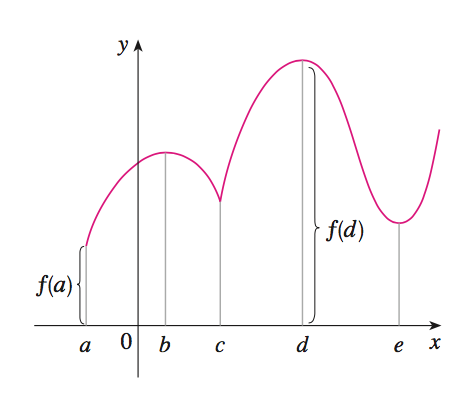
\includegraphics[scale=0.5]{images/graph-with-extrema}
\end{ex}
\vspace{-2.5in}
\begin{ex}
  Find the relative extrema of \(f(x) = 3x^4 - 4x^3 - 12x^2 +
  5\). Find the relative extrema of \(g(x) = x^3\) and \(h(x) = x +
  \frac{1}{x}\) as well.
\end{ex}
\begin{ex}
  The Hubble Space Telescope was deployed on April 24, 1990, by the
  space shuttle Discovery. A model for the velocity of the
  shuttle during this mission, from liftoff at \(t=0\) until the solid
  rocket boosters were jettisoned at \(t = 126\) s is given by \[
    v(t) = 0.001 t^3 - 0.09t^2 + 24t - 3 \text{ (in ft/s)}
  \]
  Estimate the absolute maximum and minimum values of the
  \emph{acceleration} of the shuttle between liftoff and the
  jettisoning of the boosters.
\end{ex}
%%%%%%%%%%%%%%%%%%%%%%%%%%%%%%%%%%%%%%%%%%%%%%%%%%
\end{document}
